%%% -*- TeX-master: "../main" -*-
\chapter{From Time Series to Label Sequences}
\label{cha:methods}

\begin{figure}[h]
  % Center this figure specifically because it is wider than \textwidth
  \makebox[\textwidth][c]{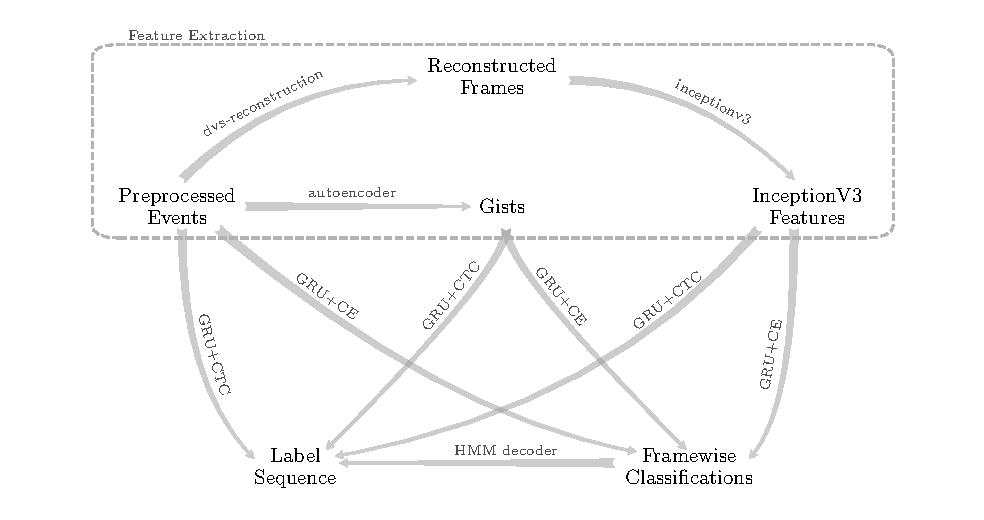
\includegraphics{figures/methods/overview}}
  \caption{Overview of the methods and intermediate steps that we used to get
    from an event sequence to a label sequence}
  \label{fig:method-overview}
\end{figure}

\section{Recurrent Neural Networks}
\label{sec:rnns}

\section{Frame Reconstruction}
\label{sec:frame-reconstruction}

\section{Feature Extraction with an InceptionV3 Network}
\label{sec:inceptionv3}

\section{Representation Learning with an Autoencoder}
\label{sec:autoencoder}

\section{Framewise Classification}
\label{sec:framewise}

\section{Hidden Markov Model Decoding}
\label{sec:hmm}

\section{Connectionist Temporal Classification}
\label{sec:ctc}

Training with categorical cross entropy tries to categorize short windows of events correctly.
However, this is not actually what we want and may also be impossible to do.
For example, the gestures extend-index-finger and tap-index-finger start the exact same way, so the first few events are not distinguishable.
With CTC we might be able to get the network to stay quiet until it is sure, which type of gesture it is, instead of forcing it to predict one of them at inappropriate times.
